
\documentclass[refman]{article}
\usepackage[utf8]{inputenc}
\usepackage[english]{babel}


%

\usepackage{colortbl}
\usepackage{epigraph}
\usepackage{fancyhdr}
\usepackage{graphicx}
\usepackage{hhline}
\usepackage{biblatex}

\usepackage[procnames]{listings}
\usepackage{longtable}
\usepackage{tikz}
\usepackage{subcaption}
\usepackage{xcolor}
\usepackage{wrapfig}
\usepackage[nottoc,numbib]{tocbibind}
%
%\usepackage[T1]{fontenc}
\usepackage{lmodern}

\usepackage{amsfonts}
\usepackage{amsmath}
\usepackage{amsthm}
\usepackage{mathtools}

\usepackage{geometry}
 \geometry{
 a4paper,
 left=30mm,
 top=30mm,
 }
\pagestyle{fancy}

\newcommand{\idx}{\text{idx}}

\DeclarePairedDelimiter\ceil{\lceil}{\rceil}
\DeclarePairedDelimiter\floor{\lfloor}{\rfloor}

\theoremstyle{definition}
\newtheorem*{formula}{Formula}

\usepackage[document]{ragged2e}

\begin{document}

\begin{align*}
	u(x) := \prod_{l=1}^d x_l \sin (\kappa \pi x_l)
\end{align*}

\begin{align*}
	f(x) = - \Delta u(x) = -\sum_{l = 1}^d \frac{\partial^2 u}{\partial x_l^2} (x)
\end{align*}

\begin{align*}
	f_{d=1} (x_1) =& \kappa \pi \left( \kappa \pi x_1 \sin ( \kappa \pi x ) - 2 \cos( \kappa \pi x_1) \right) \\
%	
	f_{d=2} (x_1, x_2) =& \kappa \pi x_2 \sin( \kappa \pi x_2) \left(  \kappa \pi x_1 \sin(\kappa \pi x_1) - 2 \cos ( \kappa \pi x_1) \right) + \\ 
	& \kappa \pi x_1 \sin( \kappa \pi x_1) \left(  \kappa \pi x_2 \sin(\kappa \pi x_2) - 2 \cos ( \kappa \pi x_2) \right) \\
%
	f_{d=3} (x_1, x_2, x_3) =& \kappa \pi x_2 \sin( \kappa \pi x_2) \kappa \pi x_3 \sin(\kappa \pi x_3)  \left(  \kappa \pi x_1 \sin(\kappa \pi x_1) - 2 \cos ( \kappa \pi x_1) \right) + \\
	& \kappa \pi x_1 \sin( \kappa \pi x_1) \kappa \pi x_3 \sin(\kappa \pi x_3)  \left(  \kappa \pi x_2 \sin(\kappa \pi x_2) - 2 \cos ( \kappa \pi x_2) \right) + \\
	& \kappa \pi x_1 \sin( \kappa \pi x_1) \kappa \pi x_2 \sin(\kappa \pi x_2)  \left(  \kappa \pi x_3 \sin(\kappa \pi x_3) - 2 \cos ( \kappa \pi x_3) \right)
\end{align*}

\begin{figure}[h]
	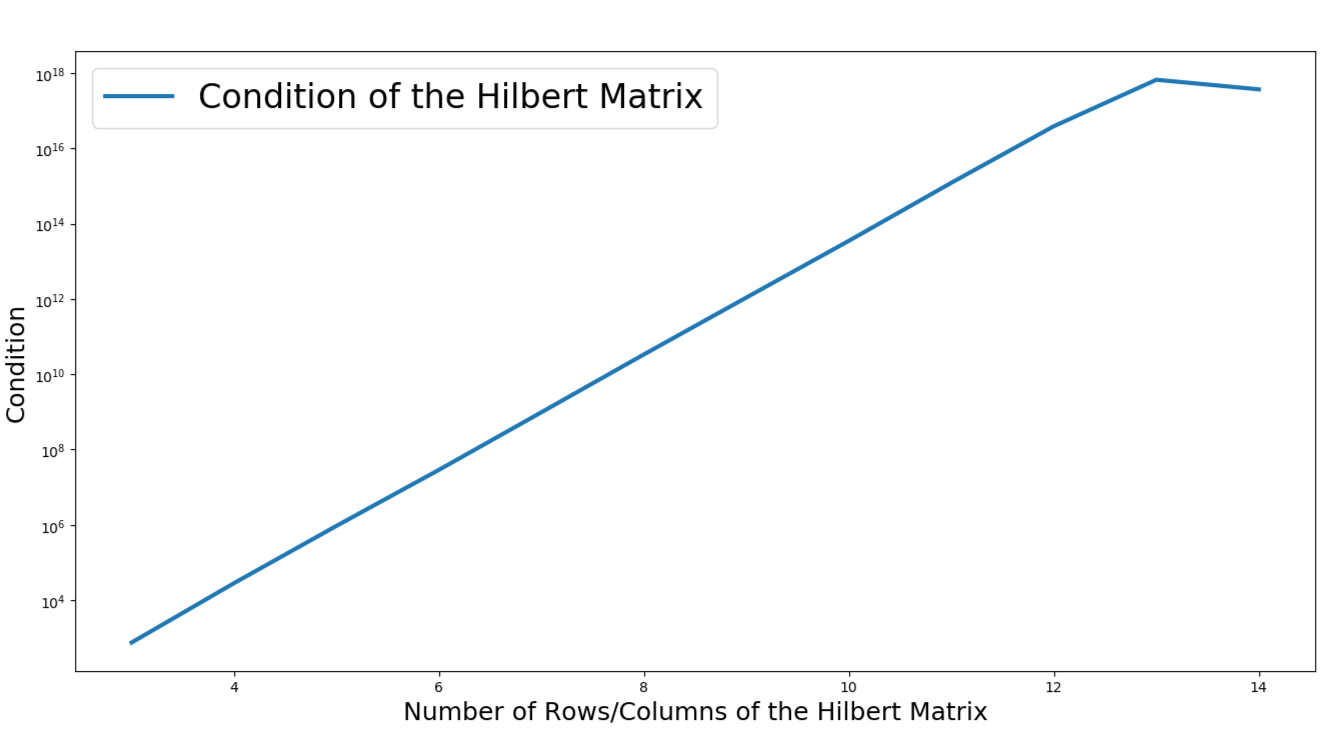
\includegraphics[width=\linewidth]{graphics/hilbert_condition.png}
	\caption{Figure 1}
	\label{fig:boat1}
\end{figure}

\end{document}